\section*{Introduction}

La quatrième révolution industrielle, aussi appellée Industrie 4.0, a inauguré
l'intégration numérique des chaînes de production et des appareils intelligents
et connectés pour des systèmes de fabrication plus efficaces. En parallèle, la
recherche en intelligence artificielle a connu une croissance substantielle,
avec des avancées significatives en matière de systèmes d'apprentissage
automatique ou apprentissage machine.\\

Les réseaux de neurones profonds modernes offrent un potentiel significatif pour
renforcer les capacités des appareils connectés. Cependant, le déploiement  de
ces réseaux de neurones sur ces appareils présente un défi en raison de la
puissance de calcul et de l'espace mémoire limités. Pour palier à ce problème de
ressources, il est possible de déplacer les calculs vers le cloud, c'est à dire
vers de puissants serveurs distants. Cepdnant, traiter les données locatlement
présente des avantages: cela garantit une meilleure confidentialité des données,
limite les communications et par conséquent réduit la bande passante utilisée,
augmente la réactivité en réduisant la latence car il n'y a pas de transfers
réseau, et cela permet de construire des appareils capables de fonctionner en
autonomie.\\

Le travail de cette thèse CIFRE est réalisé dans le contexte industriel avec
Netatmo, une entreprise française spécialisée dans les appareils connectés
intelligents. Netatmo commercialise notamment des caméras d'interrieur et
d'extérieure capable d'effectuer de la détection d'objet de de la reconnaissance
faciale. Ces tâches sont réalisés directement sur la caméra afin de garantir la
confidentialité des données et de proposer des produits sans abonnements (les
coûts du cloud n'étant pas à couvrir). Netatmo utilise des réseaux de neurones
profonds pour ces tâches. Cependant, bien que performants, ces derniers sont
gourmands en ressources et ne peuvent pas être déployés tels quels sur les
caméras. Faire fonctionner ces réseaux de neurones directement sur les caméras
présente donc un cas convaincant pour le développement de réseaux de neurones
allégés, adaptés aux appareils connectés. Ces réseaux légers doivent atteindre
des niveaux de performance comparable à leurs homologues plus grands tout en
étant nettement moins gourmands en taille et en exigences de calcul.\\

Cette thèse aborde le défi de la compression des réseaux de neurones profonds à
travers l'élagage, une technique qui vise à réduire la taille d'un réseau de
neurones en supprimant les paramètres redondants ou inutiles. Elle présente en
particulier une méthode de reparametrisation des poids couplé à une fonction de
coût représentatn un budget qui permet d'éviter le réentrainement des poids
élagués, ainsi qu'une méthide de rééchantillonnage stochastique des poids qui ne
nécessitent pas d'entrainement des poids du réseau pour déterminer leur
pertinence au sein de l'architecture finale. Cela permet de rechercher une
topologie à la fois légère et performante à l'intérieur du réseau original sans
entrainer les poids.\\

\section*{Apprentissage profond et réseaux de neurones}

L'appentissage profond est un sous-domaine de l'apprentissage automatique qui se
concentre sur les réseaux de neurones profonds, un évolution des réseaux de
neurones artificiels. Ces derniers visent à apprendre une représentation des
données à partir d'informations non structurées telles que les images, le texte
ou l'audio. Ces réseaux ont été exploités dans diverses tâches, comme la
reconnaissance d'images et de parole, le traitement du langage naturel, la
détection d'objets entre autres
\cite{DBLP:conf/icml/AmodeiABCCCCCCD16,DBLP:conf/nips/RenHGS15,DBLP:conf/nips/KrizhevskySH12,
  DBLP:conf/emnlp/BudzianowskiV19,DBLP:conf/cvpr/HeZRS16,jumper2021highly}.
Historiquement, les réseaux de neurones artificiels ont cherché à reproduire les
réseaux neuronaux biologiques \cite{mcculloch1943logical} avant d'évoluer vers
des architectures plus complexes composées de blocs de base présentés dans la
suite.

\subsection*{Architectures Pionnières}\label{sec:dlo:early_architectures}

% Cette section présente le perceptron \cite{rosenblatt1958perceptron} et le
% \acl{MLP}, deux architectures fondamentales qui ont conduit au développement des
% \acp{DNN}.

Le premier modèle mathématique cherchant à reproduire le comportement d'un
neurone est le \emph{perceptron} \cite{rosenblatt1958perceptron}. Il s'agit d'un
modèle de neurone artificiel introduit par \citeauthor{rosenblatt1958perceptron}
qui est capable d'apprendre une limite de décision linéaire. Il est composé de
$n$ entrées $x_i$ pondérées par des poids $w_i$, qui sont ensuite passées par
une fonction d'activation non linéaire $g$. Sa formulation mathématique est
définie par l'équation \cref{eqn:dlo:perceptron}:

\begin{equation}
  \label{eqn:dlo:perceptron}
  \hat{y} = g(\sum_{i=1}^{n} w_i \cdot x_i + b)
\end{equation}

Une évolution directe du perceptron est le perceptron multi-couches qui est
composé de plusieurs couches de perceptrons aussi appelés neurones
\cite{rumelhart1986learning}. Il s'agit du type le plus simple de réseau de
neronnes artificiel. Une représentation du \ac{MLP} avec une couche cachée est
donnée dans \cref{fig:dlo:mlp}. Contrairement au perceptron, le perceptron
multicouche peut apprendre une frontière de décision non linéaire. Sa
formulation vectorielle est donnée par l'équation \cref{eqn:dlo:mlp}, où $g_i$
represente la fonction d'activation de la couche $i$, $\mathbf{w}_i$ les poids,
$\mathbf{b}_i$ le biais, et $\mathbf{x}$ l'entrée.

\begin{equation}
  \label{eqn:dlo:mlp}
  \hat{\mathbf{y}} = g_2(\mathbf{w}_2^T \cdot  g_1(\mathbf{w}_2^T \cdot \mathbf{x} + \mathbf{b}_1) + \mathbf{b}_2)
\end{equation}

\begin{figure}[htbp]
  \centering
  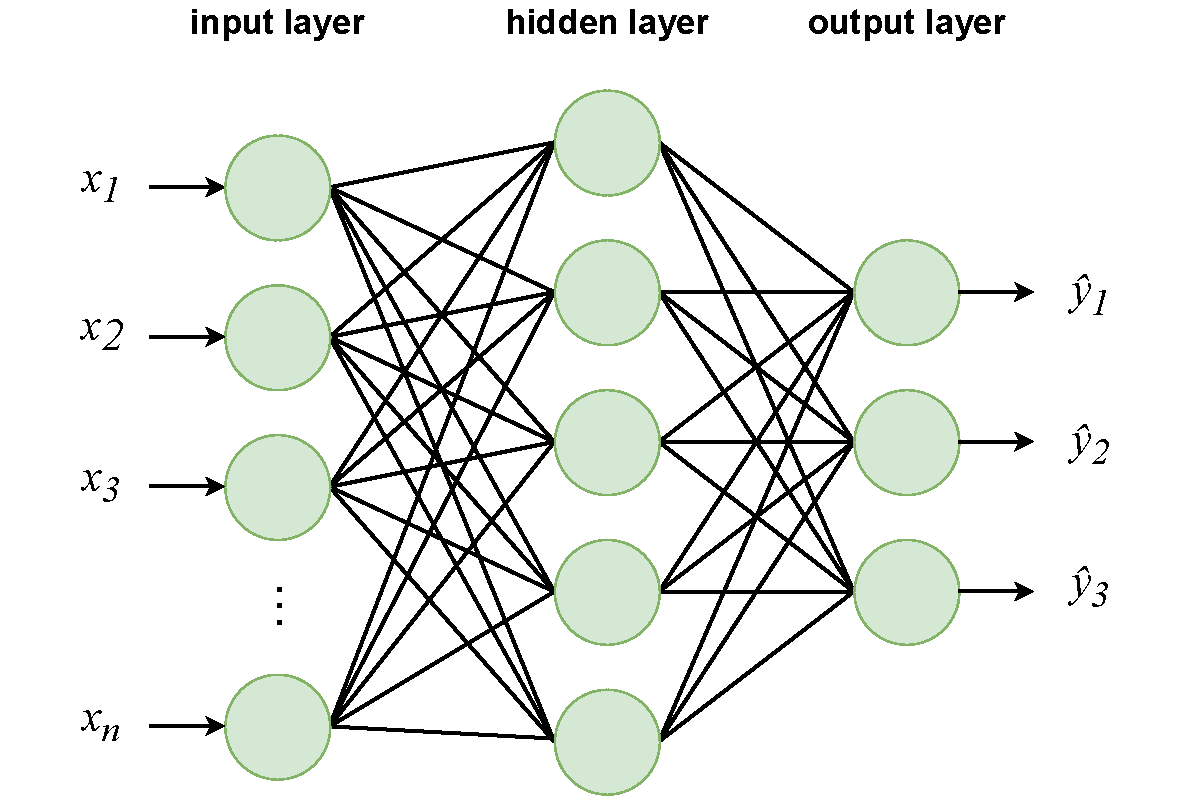
\includegraphics[width=0.5\textwidth]{./chapter_dlo/assets/mlp_scheme.pdf}
  \caption{Représentation d'un perceptron multi-couches avec une couche cachée.}
  \label{fig:dlo:mlp}
\end{figure}


\subsection*{Entrainement du réseau de neurones}\label{sec:dlo:training}

L'entraînement des réseaux neuronaux consiste en l'optimisation d'une fonction
de coût. Celle-ci quantifie la différence entre la sortie du réseau et la sortie
attendue. L'optimisation est faite en ajustant les paramètres du réseau,
également appelés poids et utilise principalement l'algorithme de
\emph{rétropropagation} \cite{rumelhart1986learning} pour calculer les gradients
et l'algorithme de descente de gradient stochastique
\cite{robbins1951stochastic} pour mettre à jour les poids.\\

Formellement, un réseau de neurones est une fonction de correspondance d'un
espace d'entrée $\mathcal{X}$ vers un espace de sortie $\mathcal{Y}$,
caractérisée par des paramètres $\theta$, appelés \emph{poids}. L'objectif est
d'ajuster $\theta$ pour que la sortie du réseau, $\hat{y}$, soit la plus proche
possible de la sortie réelle $y$ pour une entrée $X$ donnée. Dans le cas d'une
tâche de classification, la fonction de coût la plus courante est l'entropie
croisée qui s'écrie comme suit:

\begin{equation}
  \label{eqn:dlo:cross_entropy}
  \mathcal{L}_{\text{classif.}}(y, \hat{y}) = - \sum_{i=1}^{C} y_i \cdot \log(\hat{y}_i)
\end{equation}

\noindent où $C$ est le nombre de classes, $\mathcal{L}$ est la fonction de
coût, $y$ est la sortie attendue, aussi appelée \emph{vérité terrain}, et
$\hat{y}$ est la sortie prédite. Afin de réduire le risque de surapprentissage,
on adjoint à la fonction de coût une régularisation $\mathcal{R}(\theta)$ basée
sur les poids qui containt leur magnitude. $\mathcal{R}$ est généralement la
norme $\ell_1$ ou $\ell_2$ des poids. La fonction de coût finale est donc
$\mathcal{L} = \mathcal{L}_{\text{classif.}}(y,\hat{y}) +
  \mathcal{R}(\theta)$.\\


L'optimisation de cette fonction de coût est réalisée de manière itérative en
utilisant l'algorithme de descente de gradient stochastique. Cet algorithme
calcule le gradient de la fonction de coût par rapport aux paramètres du réseau
et met à jour les poids en fonction de ce gradient. La descente de gradient
stochastique est une variante de la descente de gradient classique qui calcule
le gradient sur l'ensemble des données d'entraînement. La descente de gradient
stochastique calcule le gradient sur un sous ensemble de données, appelé
mini-lot. Les poids sont mis à jour après chaque mini-lot de la manière
suivante :

\begin{equation}
  \label{eqn:dlo:sgd}
  \theta_{t+1} = \theta_t - \eta \cdot \nabla_{\theta_t} \mathcal{L}
\end{equation}

\noindent Ici, $\theta_t$ est le poids à l'itération $t$, $\eta$ est le taux
d'apprentissage qui contrôle la taille du pas de mise à jour des poids et
$\nabla_{\theta_t} \mathcal{L}$ est le gradient de la fonction de coût par
rapport aux paramètres du réseau. Ce dernier est calculé en utilisant le
théorème de dérivation des fonctions composées en tendem avec l'algorithme de
rétropropagation du gradient pour calculer le gradient de chaque poids de
manière efficace \cite{rumelhart1986learning}.\\

\subsection*{Architectures Convolutionnelles pour la Vision par Ordinateur}
Les Réseaux de neurones Convolutifs se sont imposés comme des architectures
performantes dans le domaine de la vision par ordinateur, notamment pour la
classification d'images. Leur efficacité réside dans leur capacité à apprendre
de manière hiérarchique des caractéristiques visuelles abstraites grâce aux
couches de convolution. Ils sont composé de différentes briques de bases
organisés en architectures. Ces briques de basent sont les suivantes:\\

\begin{itemize}
  \item \emph{Couche de convolution.} Cette couche effectue des convolutions
        spatiales sur les données d'entrée à l'aide de filtres, dont les poids sont
        entraînables, permettant d'extraire des caractéristiques allant d'un faible
        niveau d'abstraction (bords, coins, textures) à un haut niveau (objets,
        parties d'objets).
  \item \emph{Couche entièrement connectée.} Souvent situées à la fin des
        réseaux de neurones convolutifs, ces couches agissent comme des
        classificateurs. Elles réalisent des transformations non linéaires des
        caractéristiques extraites et se présente sous la forme de produits
        matriciels dont les vecteurs sont les caractéristiques extraites et les
        matrices les poids de la couche.
  \item \emph{Fonction d'activation.} Ces fonction, appliquées aux sorties des
        couches précédemment décrites, introduisent de la non-linéarité dans le
        réseau et permettent au modèle d'apprendre des motifs plus complexes. La
        fonction \ac{ReLU} ($\max(x,0)$) est la plus couramment utilisée. Elle
        présente les avantages d'être simple à calculer et de ne pas saturer
        pour des valeurs de sortie élevées. La sortie de cette couche est
        appelée l'\emph{activation}, en référence à l'activation biologique des
        neurones.
  \item \emph{Sous-échantillonnage (Pooling).} Cette couche réduit la dimension
        spatiale des représentations, diminuant ainsi le nombre de paramètres et les
        calculs dans les couches suivantes. Deux types courants sont le \emph{max
          pooling} et l'\emph{average pooling}. Le premier consiste à prendre la
        valeur maximale dans une fenêtre de taille $k \times k$ et le second à
        prendre la valeur moyenne.
  \item \emph{Normalisation par lot.} La normalisation par lot permet de lutter
        contre le changement de distribution entre les données d'entrainement et
        celles d'évaluation, accélérant ainsi l'entrainement et améliorant la
        généralisation. Elle est appliquée après les couches de convolution ou
        entièrement connectées et normalise les activations en utilisant la
        moyenne et l'écart-type de chaque mini-lot.
  \item \emph{Dropout.} Cette technique de régularisation permet d'éviter
        le surapprentissage. Elle désactive aléatoirement une proportion de neurones
        lors de chaque itération d'entrainement, poussant le réseau à apprendre des
        représentations plus robustes.
\end{itemize}

\subsection*{Architectures Modernes}

Les réseaux de neurones convolutifs profonds modernes ont connu plusieurs
évolutions qui ont conduit à des architectures plus profondes et plus
performantes, mais toujours composées des briques de bases présentées plus haut.
Un des premiers réseau de neurones convolutifs profonds est AlexNet
\cite{DBLP:conf/nips/KrizhevskySH12} qui comporte plusieurs couches de
convolutions suivies de couches entièrement connectées. VGG16
\cite{DBLP:journals/corr/SimonyanZ14a} est une évolution d'AlexNet qui comporte
d'avantage de couches de convolutions et des filtres de plus petite taille
($3\times 3$, contre $7 \times 7$ pour AlexNet), dont l'architecture est visible
sur la \cref{fig:dlo:vgg16}. ResNet \cite{DBLP:conf/cvpr/HeZRS16} est une
architecture plus récente qui comporte des connexions résiduelles entre les
couches. Ces connexions permettent de résoudre le problème de disparition du
gradient qui se produit lors de la rétropropagation dans les réseaux profonds.
La \cref{fig:dlo:resnet} présente l'architecture de ResNet-18. L'utilisation de
connexions résiduelles ont permis, entre autre, d'augmenter la profondeur des
réseaux de neurones (c'est à dire leur nombre de couches) ainsi que leurs
performances. En conséquence de ces avancées, les tailles des réseaux de
neronnes modernes sont maintenant trop importantes pour être déployés sur des
appareils connectés.\\

\begin{figure}
\centering
\subfloat[VGG16\label{fig:dlo:vgg16}]{
  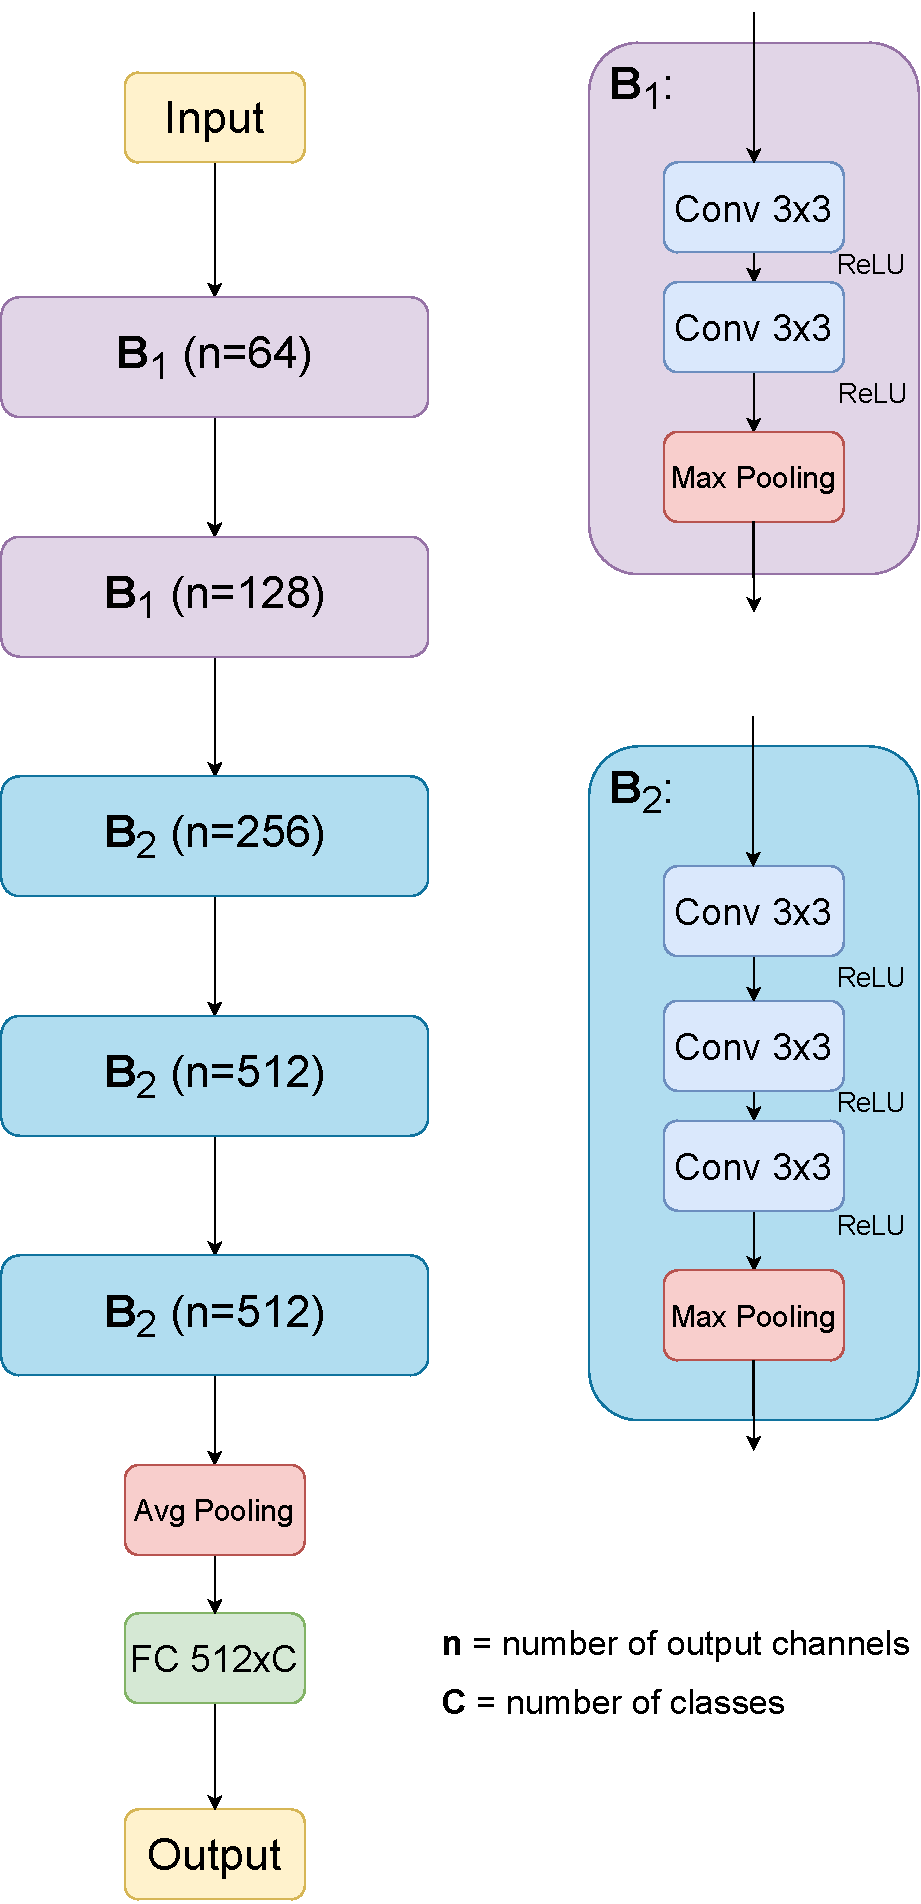
\includegraphics[width=0.3\textwidth]{./chapter_dlo/assets/vgg16_cifar.pdf}}
\hspace{0.05\textwidth}
\subfloat[ResNet-18\label{fig:dlo:resnet}]{
  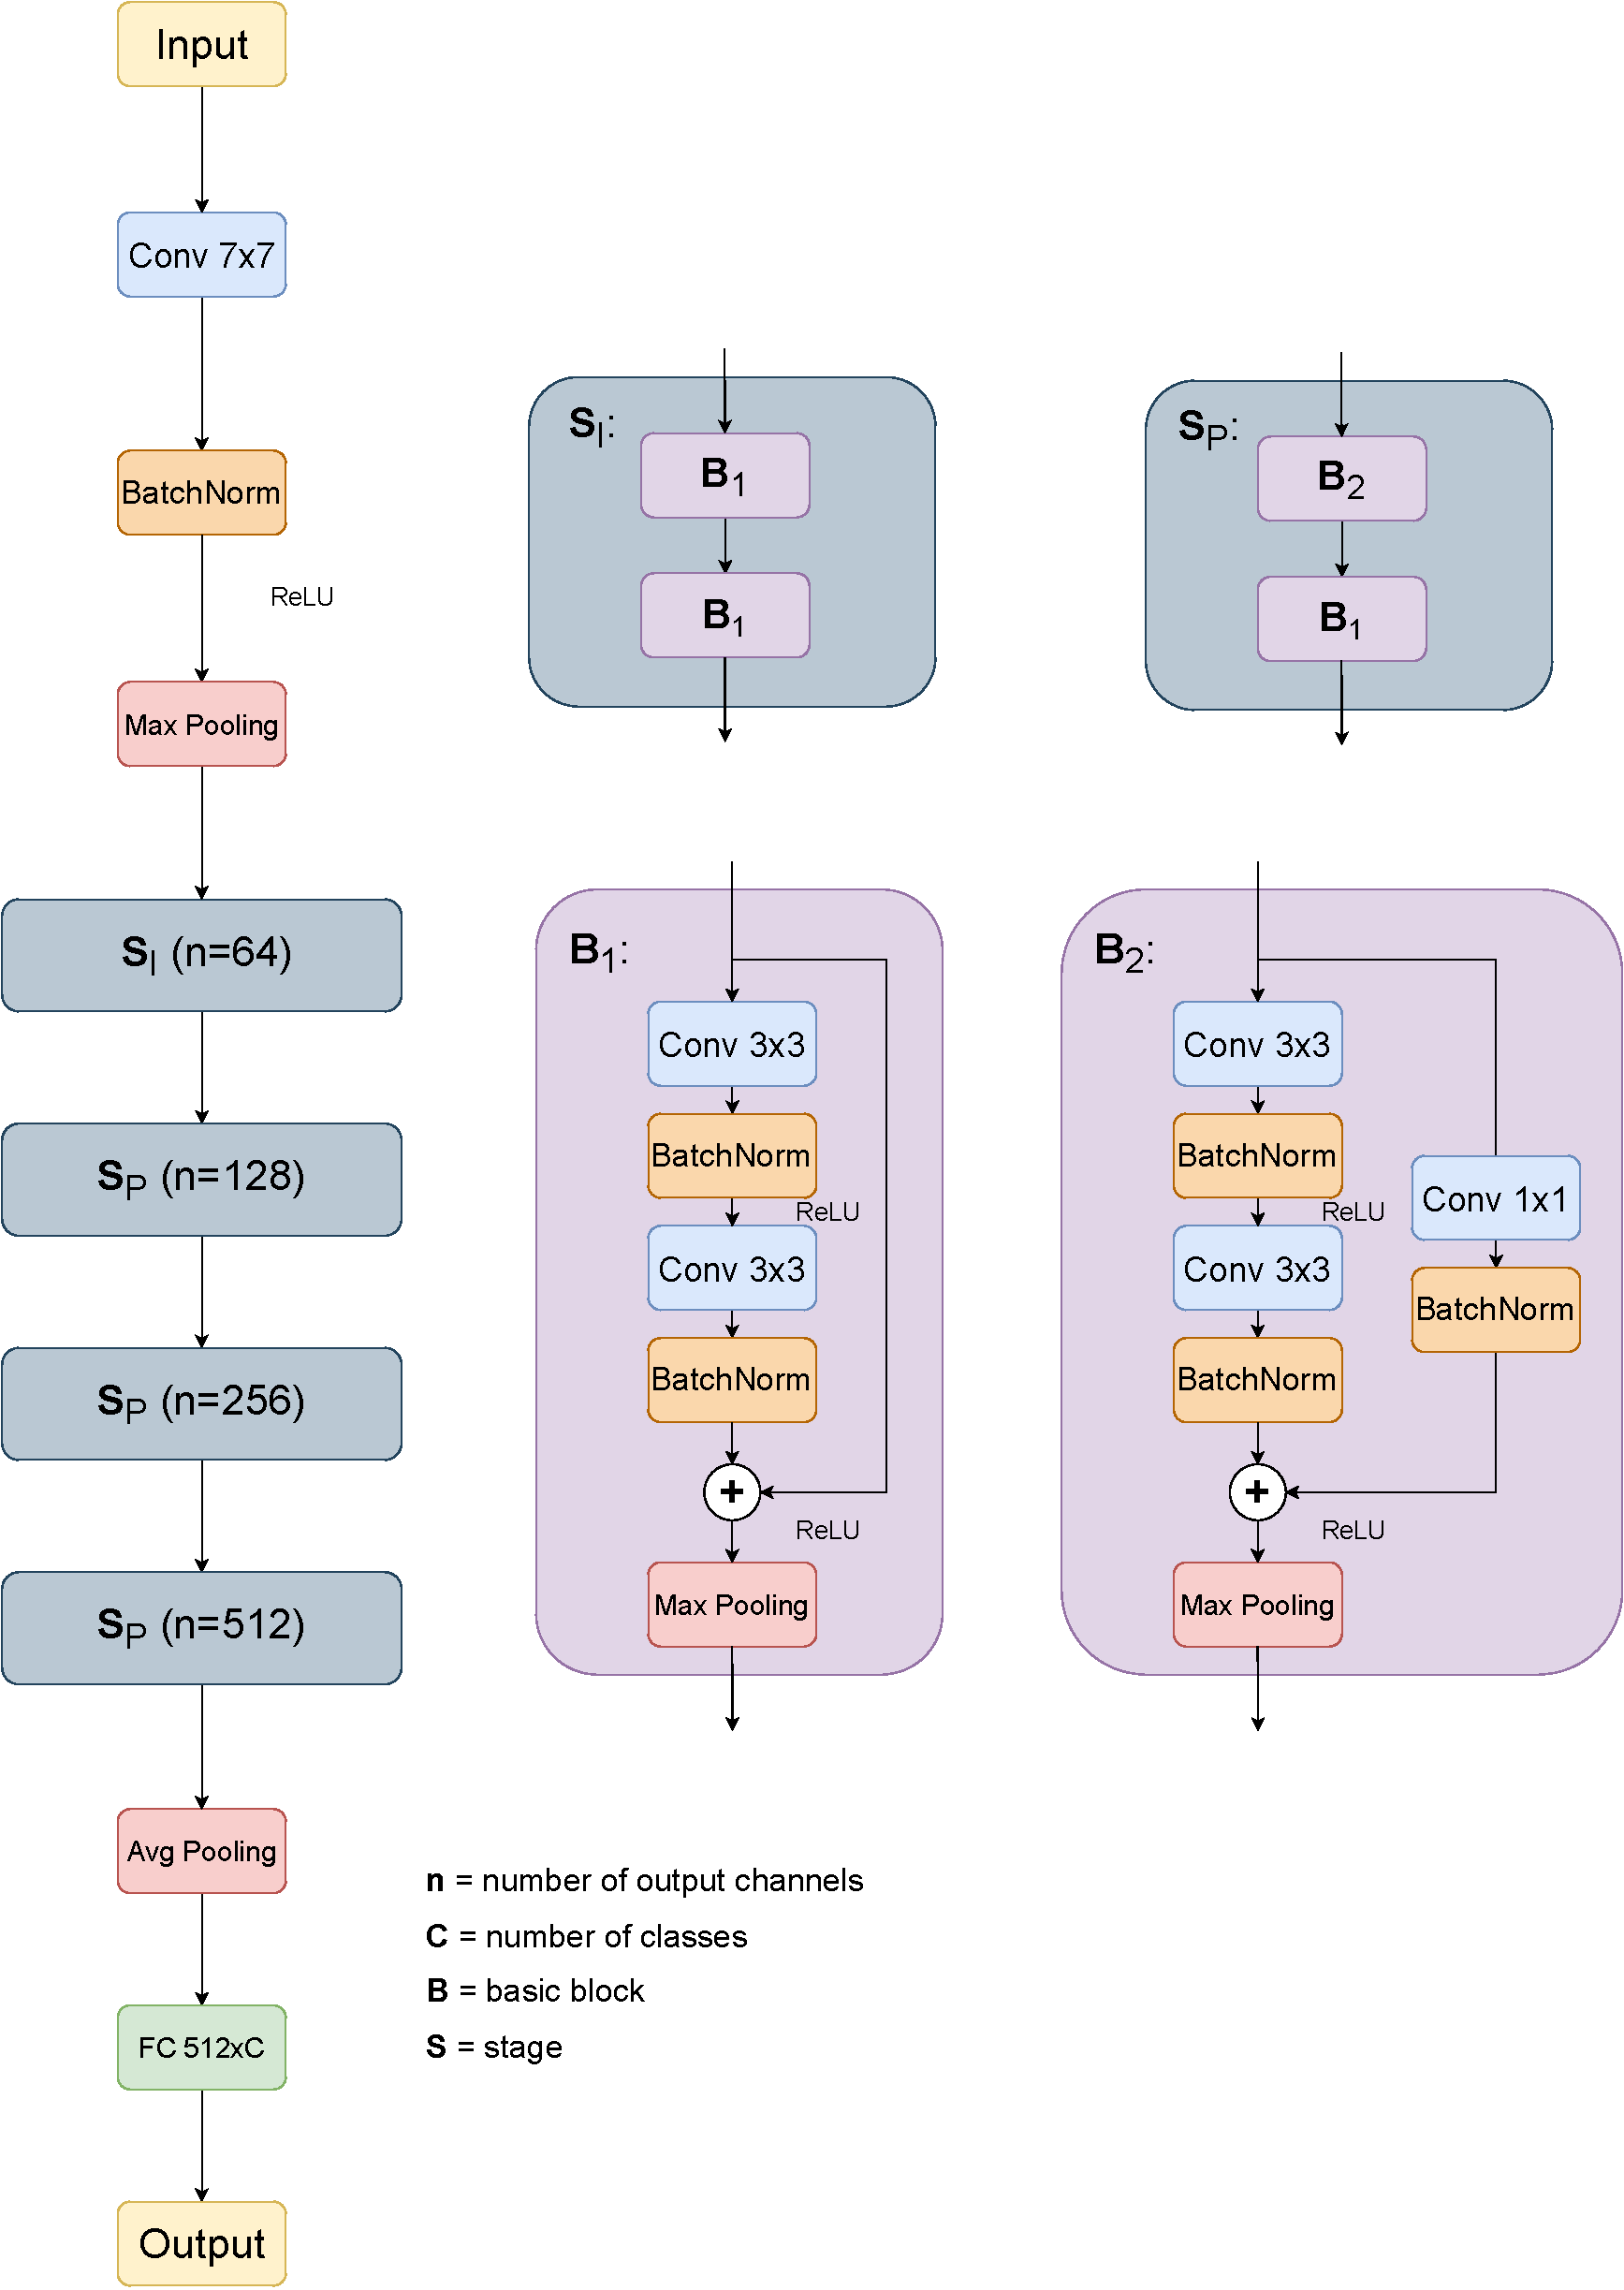
\includegraphics[width=0.5\textwidth]{./chapter_dlo/assets/resnet18.pdf}}
\caption{Architecture de réseau de neurones convolutifs modernes.}
\end{figure}


\section*{Compression et accélération de réseaux de neurones}

Les réseaux de neurones profonds modernes comportent un nombre important de
couches et de paramètres, ce qui les rend gourmands en ressources. Cela pose un
problème pour leur déploiement sur des appareils qui ont des ressources
limitées. La compression des réseaux de neurones est une solution pour réduire
la taille des réseaux et les rendre plus légers. Elle permet également de
réduire les exigences de calcul et en mémoire, ce qui est particulièrement
important pour les appareils connectés, le stockage n'étant pas le facteur
limitant. La compression des réseaux de neurones n'est cependant pas sans
conséquence sur les performances. Celles-ci peuvent s'en retrouver dégréadées.
Les méthodes de compression et d'accélération peuvent êtres réparties en
plusieurs grandes familles de méthodes :\\

\noindent \textbf{Acceleration des opérations.} Les modèles de réseaux de
neurones convolutifs sont essentiellements composés d'opérations de convolution
et de multiplication matricielle. Dès lors, accélérer ces opérations permet un
gain en temps de calcul. Les opérations matricielles peuvent être accélérées en
de différente manières. En remarquant que l'opération de convolution dans le
domaine du problème $(y = x * k)$ est une multiplication dans le domaine de
Fourier $(y_{\mathcal{F}} = x_{\mathcal{F}} \times k_{\mathcal{F}})$, il est
possible d'accélérer les convolutions en utilisant la transformée de Fourier
inverse sur la multiplication des opérandes dans le domaine de Fourier $(y =
\mathcal{F}^{-1} (x_{\mathcal{F}} \times k_{\mathcal{F}}))$
\cite{DBLP:conf/nips/ChiJM20,DBLP:journals/npl/LinY19,DBLP:conf/pkdd/PrattWCZ17}.
Il est également possible d'accélérer les multiplicatons matricielles en
optimisant directement l'ordre des opérations. C'est ce que propose de faire
l'algorithme de Strassen \cite{strassen1969gaussian}, plus tard almélioré dans
l'algorithme de Coppersmith-Winograd \cite{coppersmith1987matrix}. Ces
algorithmes décomposent récursivement une multiplication matricielle en
multiplications par blocs, qui sont ensuite réordonnés pour baisser le nombre
multiplication au prix d'un nombre d'addition accru (cependant, la complexité de
celles ci est négligeable devant celle des multiplications). On peut également
tirer parti des méthodes tout juste mentionnées pour accélérer les convolutions.
Pour ce faire, il faut transformer les opérations de convolution en
multiplication matricielle en représentant le noyeau de convolution comme une
matrice circulante \cite{DBLP:conf/iccv/ChengYFKCC15} ou une matrice de Toeplitz
\cite{gray2006toeplitz,liao2019compressing}.\\

\noindent \textbf{Paradigme Professeur-Élève.} Une des approches pour compresser
un réseau de neurones consiste à utiliser directement une petite achitecture et
a transférer les connaissances d'un réseau plus grand vers le plus petit. Le
petit réseau est alors appellé \emph{élève} et le grand réseau
\emph{professeur}. Ce procédé à été introduit par
\cite{DBLP:journals/corr/HintonVD15} \cite{DBLP:journals/corr/HintonVD15} qui
propose d'entrainer un petit réseau sur une tâche donnée et de rajouter dans à
la fonction de coût une régularisation basée sur la divergence de
Kullback-Leibler entre les sorties du petit réseau et celles du grand réseau,
également entrainé sur la même tâche. Cette régularisation permet de guider
l'élève vers les sorties du professeur. La fonction de coût totale s'écrit donc
:\\

\begin{equation}
  \mathcal{L}_{\text{totale}} = \underbrace{\mathcal{L}_{\text{CE}}(\hat{y}_{e}, y)\vphantom{\left(\frac{\hat{y}_{e}}{T}, \frac{\hat{y}_{p}}{T}\right)}}_{\text{Tâche}} +
  \lambda \frac{T^{2}}{2}\underbrace{\mathcal{L}_{\text{CE}}\left(\frac{\hat{y}_{e}}{T}, \frac{\hat{y}_{p}}{T}\right)}_{\text{Distillation}}
\end{equation}\\

\noindent où $\mathcal{L}_{\text{CE}}$ est l'entropie croisée (voir
\cref{eqn:dlo:cross_entropy}) et $\lambda\frac{T^{2}}{2}$ est un coefficient de
ponderation des 2 fonctions de coût. Cette méthode a inspiré d'autres approches
qui se basent sur le même principe : le transfer de connaissances d'un réseau à
un autre, mais en utilisant d'autres régularisations.
\citeauthor{DBLP:journals/corr/RomeroBKCGB14}
\cite{DBLP:journals/corr/RomeroBKCGB14} propose d'utiliser une norme $\ell_2$
pour quantifier l'écart des cartes d'activations entre le professeur et l'élève.
Cette méthode a été améliorée dans \cite{DBLP:conf/iclr/ZagoruykoK17} ou l'on
considère l'attention plutôt que les cartes d'activation pour transferer la
connaissance. La distillation telle que présentée dans
\cite{DBLP:journals/corr/HintonVD15} a été revisité dans
\cite{DBLP:conf/aaai/MirzadehFLLMG20}, qui propose de mettre en place un
\emph{assistant} qui est un réseau de taille intermédiaire entre l'élève et le
professeur afin de proposer une transition plus douce entre les 2 réseaux.
Enfin, une variante de l'approche professeur-élève a été présentée dans
\cite{DBLP:conf/cvpr/ZhangXHL18} où tous les réseaux sont à la fois élève et
professeur.\\


\noindent \textbf{Architecture spécifiques.} Afin de permettre le déploiement de
réseaux de neurones sur des appareils aux ressources limitées, des travaux de
recherche se sont employés à concevoir des architectures spécifiques basées sur
de nouvelles briques de bases qui permettent de réduire la taille des réseaux
tout en conservant leurs performances. MobileNet
\cite{DBLP:journals/corr/HowardZCKWWAA17} est le parfait exemple de ce type de
réseau. Il est composé de \emph{convolutions séparables en profondeurs} qui
permettent de réduire le nombre de paramètres et de calculs. Les convolutions
séparables en profondeurs sont composées de 2 opérations : une convolution
\emph{en profondeur} et une convolution \emph{en largeur}. La convolution en
profondeur est une convolution spatiale classique, tandis que la convolution en
largeur est une convolution $1 \times 1$ qui permet de réduire le nombre de
canaux. D'autres briques de bases ont été proposées dans les achitectures
SqueezeNet \cite{DBLP:journals/corr/IandolaMAHDK16} et ShuffleNet
\cite{ZhangShuffleNet,MaShuffleNetV2}. Le premier introduit les \emph{fire
modules} qui sont des couches de convolution qui mélangent différentes tailles
de noyeau de convolution, afin de préserver l'expressivité du réseau tout en
limitant le nombre de paramètres avec des noyeau plus petits. Le second propose
le concept de \emph{channel shuffle} couplé à des convolutions groupées, ce qui
permet de partager les caractéristiques apprises entre les groupes. Si ces
architectures sont performantes, elles ont été conçues à la main par des humains
et ont nécessité beaucoup de travail et d'expertise. Il est possible d'obtenir
d'autres architecture de manière automatique en utilisant des méthodes de
recherche d'architecture. Celles-ci sont basées sur des algorithmes
d'optimisation qui cherchent à trouver la meilleure architecture pour une tâche
donnée. Parmi ces méthodes, on peut citer les algorithmes génétiques
\cite{DBLP:conf/icml/RealMSSSTLK17} et les algorithmes de recherche bayésienne
\cite{DBLP:conf/nips/BergstraBBK11}. D'autres méthodes sont basées sur des
relaxations continue du problème et sont optimisées avec une descente de
gradient \cite{DBLP:conf/iclr/LiuSY19}.\\

\noindent \textbf{Compression d'architectures existantes.} \lipsum[2] \\



\section*{Élagage par reparametrisation avec régularisation basée sur le budget}

\section*{Entrainement de masques pour échantillonnage stochastique des poids}

\section*{Conclusion}